\chapter{RESULT AND DISCUSSION}


\section{Experiment Setup}

All experiments for the proposed MorphAI system were conducted using a
PyTorch-based deep learning environment with GPU acceleration. The model
was trained using Automatic Mixed Precision (AMP) to improve computational
efficiency and reduce GPU memory usage. Training was performed for five
epochs on a dataset containing more than 16,800 facial images. Table
~\ref{tab:hardware} summarises the hardware and software environment used
for model training and evaluation.

\begin{table}[h!]
\centering
\renewcommand{\arraystretch}{1.1}
\begin{tabular}{|l|l|}
\hline
\textbf{Component} & \textbf{Specification} \\ \hline
GPU & NVIDIA GeForce RTX 4050 Laptop GPU (6 GB VRAM) \\ \hline
System RAM & 16 GB \\ \hline
Operating System & Windows 11 Home \\ \hline
Python & 3.11.9 \\ \hline
PyTorch & 2.6.0 + CUDA 12.4 \\ \hline
Training Precision & Automatic Mixed Precision (AMP) \\ \hline
Training Epochs & 5 \\ \hline
Training Dataset & 16,800 facial images \\ \hline
\end{tabular}
\vspace{2pt}
\caption{Hardware and software environment used for MorphAI}
\label{tab:hardware}
\end{table}

\section{Training Configuration}
The proposed MorphAI model was trained using the modified LGNet generator
with landmark-based structural conditioning. The input image was resized
to $256 \times 256$ pixels and combined with a facial mask and landmark
heatmap to form a five-channel input. The model was trained using GPU
acceleration and Automatic Mixed Precision (AMP). The main training
configuration is summarised in Table~\ref{tab:training_config}.
% \clearpage
\begin{table}[H]
\centering
\renewcommand{\arraystretch}{1.3}
\begin{tabular}{|l|l|}
\hline
\textbf{Training Setting} & \textbf{Value} \\ \hline
Dataset & CelebA-HQ (16,800 original images) \\ \hline
Image Resolution & $256 \times 256$ \\ \hline
Model & Modified LGNet Generator \\ \hline
Input & 5-channel (RGB + Mask + Heatmap) \\ \hline
Training Epochs & 5 \\ \hline
Training Precision & Automatic Mixed Precision (AMP) \\ \hline
Training Mask & Semantic facial-region masks \\ \hline
Inference Mask & Semantic masks \\ \hline
Evaluation & PSNR, SSIM, LPIPS, FID, RMSE-log, Identity Similarity \\ \hline
\end{tabular}
\caption{Training configuration of the proposed MorphAI model}
\label{tab:training_config}
\end{table}

\noindent The model was trained for five epochs primarily due to the
computational constraints of the available hardware. Training was
performed on a single NVIDIA RTX 4050 Laptop GPU (6\,GB VRAM), using
Automatic Mixed Precision (AMP) to reduce GPU memory usage and improve
computational efficiency within this resource budget. The training and
validation losses decreased consistently throughout training, indicating
stable convergence. The loss values obtained during training are
presented in Table~\ref{tab:training_loss}.

\begin{table}[H]
\centering
\renewcommand{\arraystretch}{1.2}
\begin{tabular}{|c|c|c|c|}
\hline
\textbf{Epoch} & \textbf{Training Loss} & \textbf{Validation Loss} &
\textbf{Loss Gap} \\ \hline
1 & 0.3479 & 0.3640 & 0.0161 \\ \hline
2 & 0.3124 & 0.3284 & 0.0160 \\ \hline
3 & 0.3003 & 0.3167 & 0.0164 \\ \hline
4 & 0.2847 & 0.2983 & 0.0136 \\ \hline
5 & 0.2774 & 0.2950 & 0.0176 \\ \hline
\end{tabular}
\caption{Training and validation loss across five epochs}
\label{tab:training_loss}
\end{table}

\noindent The training loss decreased from 0.3479 to 0.2774, while the
validation loss decreased from 0.3640 to 0.2950. The relatively small and
stable training--validation gap (ranging from 0.0136 to 0.0176) indicates
stable training without a substantial increase in validation error,
suggesting the model had not begun overfitting by the fifth epoch. Based
on this consistent convergence behaviour and the available computational
budget, the fifth-epoch checkpoint was selected as the final model for
evaluation. Training was not extended beyond five epochs, so no claim is
made regarding whether additional epochs would have produced further
improvement or diminishing returns.

\subsection{Ablation Consideration: Landmark Heatmap Conditioning}
The contribution of landmark heatmap conditioning is discussed based on the model 
architecture and the overall reconstruction results reported in this chapter, rather 
than through a separate controlled experiment. A dedicated ablation study — training 
an identical LGNet variant without the landmark heatmap channel, under the same 
dataset, epoch budget, and evaluation protocol — was not conducted for this project 
due to GPU and time constraints (a single 6\,GB VRAM GPU and a five-epoch training 
budget). The comparison against the LaMa baseline in Table 5.5, which does not use 
landmark conditioning at all, offers indirect evidence that the added structural 
guidance contributes to MorphAI's stronger PSNR, SSIM, and identity-similarity scores, 
but a same-architecture, single-variable ablation is left as future work.

\subsection{Quantitative Evaluation}

Semantic region-wise evaluation was performed on six facial regions
using the same 2,800 held-out facial images. Each image was evaluated
with respect to each of the six facial regions, resulting in
$2,800 \times 6 = 16,800$ region-specific evaluation samples. As shown in Table~\ref{tab:semantic_region},
LGNet generally achieves higher PSNR, SSIM, identity similarity, and lower
RMSE-log and FID than LaMa. LGNet also shows particularly strong performance
for the mouth and eye regions. LPIPS is lower for LaMa in several regions,
indicating that LGNet does not outperform the baseline on every metric.
Overall, the results demonstrate strong structural and identity preservation
by the proposed LGNet model.

\begin{table}[H]
\centering
\renewcommand{\arraystretch}{1.25}
\resizebox{\textwidth}{!}{%
\begin{tabular}{|l|l|c|c|c|c|c|c|}
\hline
\textbf{Region} & \textbf{Model} & \textbf{PSNR $\uparrow$} &
\textbf{SSIM $\uparrow$} & \textbf{LPIPS $\downarrow$} &
\textbf{ArcFace ID $\uparrow$} & \textbf{RMSE-log $\downarrow$} &
\textbf{FID $\downarrow$} \\ \hline

Left Eyebrow & LGNet & 42.36 dB & 0.9932 & 0.0061 & 0.9880 & 0.0058 & 0.2439 \\ \hline
Left Eyebrow & LaMa  & 42.10 dB & 0.9812 & 0.0025 & 0.9726 & 0.0061 & 0.1581 \\ \hline

Right Eyebrow & LGNet & 42.27 dB & 0.9931 & 0.0062 & 0.9869 & 0.0059 & 0.2422 \\ \hline
Right Eyebrow & LaMa  & 42.03 dB & 0.9811 & 0.0026 & 0.9690 & 0.0062 & 0.1549 \\ \hline

Left Eye & LGNet & 41.17 dB & 0.9938 & 0.0051 & 0.9966 & 0.0067 & 0.2491 \\ \hline
Left Eye & LaMa  & 39.97 dB & 0.9819 & 0.0032 & 0.9880 & 0.0083 & 0.7603 \\ \hline

Right Eye & LGNet & 41.14 dB & 0.9938 & 0.0051 & 0.9963 & 0.0067 & 0.2401 \\ \hline
Right Eye & LaMa  & 40.05 dB & 0.9819 & 0.0031 & 0.9869 & 0.0082 & 0.6960 \\ \hline

Mouth & LGNet & 39.87 dB & 0.9947 & 0.0032 & 0.9886 & 0.0081 & 0.5940 \\ \hline
Mouth & LaMa  & 34.59 dB & 0.9734 & 0.0090 & 0.9497 & 0.0142 & 2.3734 \\ \hline

Nose & LGNet & 39.09 dB & 0.9882 & 0.0092 & 0.9353 & 0.0080 & 0.7947 \\ \hline
Nose & LaMa  & 37.53 dB & 0.9754 & 0.0077 & 0.8660 & 0.0094 & 1.1818 \\ \hline

\end{tabular}%
}
\caption{Semantic region-wise evaluation of MorphAI (LGNet) and LaMa on 2,800 samples per region}
\label{tab:semantic_region}
\end{table}

\noindent The final model was evaluated using pixel-level, perceptual, and identity
metrics. The evaluation results were stored in JSON files, including
\texttt{metrics.json}. A separate set of results was generated
for comparison with the LaMa baseline.

\begin{table}[H]
\centering
\renewcommand{\arraystretch}{1.3}
\begin{tabular}{|l|c|c|}
\hline
\textbf{Metric} & \textbf{MorphAI (LGNet)} & \textbf{LaMa} \\ \hline
PSNR $\uparrow$ & 40.99 dB & 39.38 dB \\ \hline
SSIM $\uparrow$ & 0.9928 & 0.9792 \\ \hline
LPIPS $\downarrow$ & 0.0058 & 0.0047 \\ \hline
Identity Similarity $\uparrow$ & 0.9819 & 0.9554 \\ \hline
RMSE-log $\downarrow$ & 0.0069 & 0.0087 \\ \hline
FID $\downarrow$ & 0.1398 & 0.2466 \\ \hline
\end{tabular}
\caption{Quantitative comparison between MorphAI and LaMa}
\label{tab:morphai_lama}
\end{table}

\noindent MorphAI outperforms the LaMa baseline on PSNR, SSIM, identity similarity, 
RMSE-log, and FID, while LaMa achieves a slightly lower LPIPS score. Overall, these 
results indicate that the proposed landmark-conditioned LGNet provides strong 
reconstruction quality while maintaining facial identity.

\subsection{Discussion of LPIPS and Identity Preservation}
MorphAI does not outperform LaMa on every evaluation metric. LaMa achieves a slightly 
lower LPIPS score (0.0047 vs. 0.0058), indicating a lower perceptual feature distance 
according to the LPIPS metric. However, MorphAI achieves better PSNR, SSIM, ArcFace 
identity similarity, RMSE-log, and FID. This indicates that MorphAI provides stronger 
pixel-level reconstruction, structural consistency, and identity preservation, while 
LaMa has an advantage according to LPIPS.

\noindent This difference can be explained by what each metric is actually sensitive to. PSNR 
and SSIM measure pixel-level and structural similarity directly against the ground-truth 
image, and both reward MorphAI's landmark-conditioned reconstructions for closely 
matching the original facial structure. ArcFace identity similarity specifically rewards 
preservation of identity-discriminative features, which MorphAI's identity loss directly 
optimizes for during training. LPIPS, in contrast, measures similarity in a learned deep 
perceptual feature space that is more sensitive to fine-grained texture and stylistic 
detail than to precise structural or identity accuracy. It is likely that MorphAI's 
landmark and identity losses push the generator toward structurally and identity-accurate 
reconstructions, which can slightly reduce fine textural variation compared to LaMa's 
purely context-driven inpainting -- a difference LPIPS is more sensitive to than PSNR 
or SSIM.

\noindent The region-wise results in Table~\ref{tab:semantic_region} support this discussion. In the 
mouth region, for example, MorphAI achieves 39.87\,dB PSNR, 0.9947 SSIM, and 0.9886 
identity similarity, compared with LaMa's 34.59\,dB, 0.9734, and 0.9497, respectively. 
Therefore, the results demonstrate a metric-specific trade-off rather than universal 
superiority of one model: MorphAI prioritizes structural and identity fidelity, while 
LaMa's context-based inpainting produces marginally lower LPIPS distance in some regions.

\noindent Region-wise evaluation was also performed for the eyes, eyebrows, nose, and 
mouth. These results are stored in the \texttt{lama\_comparison} JSON files and provide 
additional analysis of performance across different facial regions.


\section{Software Development Approach}

\noindent The MorphAI project follows the Agile Software Development Life
Cycle (SDLC), where development is carried out through iterative stages.
Each iteration involves planning, implementation, testing, review, and
refinement. This approach allows individual components to be developed
and improved based on intermediate experimental results.

\noindent The development began with literature review, dataset
preparation, image preprocessing, and facial landmark extraction.
Subsequent iterations focused on facial mask generation, landmark
heatmap conditioning, LGNet architecture modification, and ArcFace
identity-preservation integration. The final stages focus on model
training, evaluation, comparison, and refinement. Agile was selected
because the project involves continuous experimentation with the
dataset, model architecture, and loss functions, allowing changes to be
made incrementally without affecting the entire system.
    \begin{figure}[H]
        \centering
        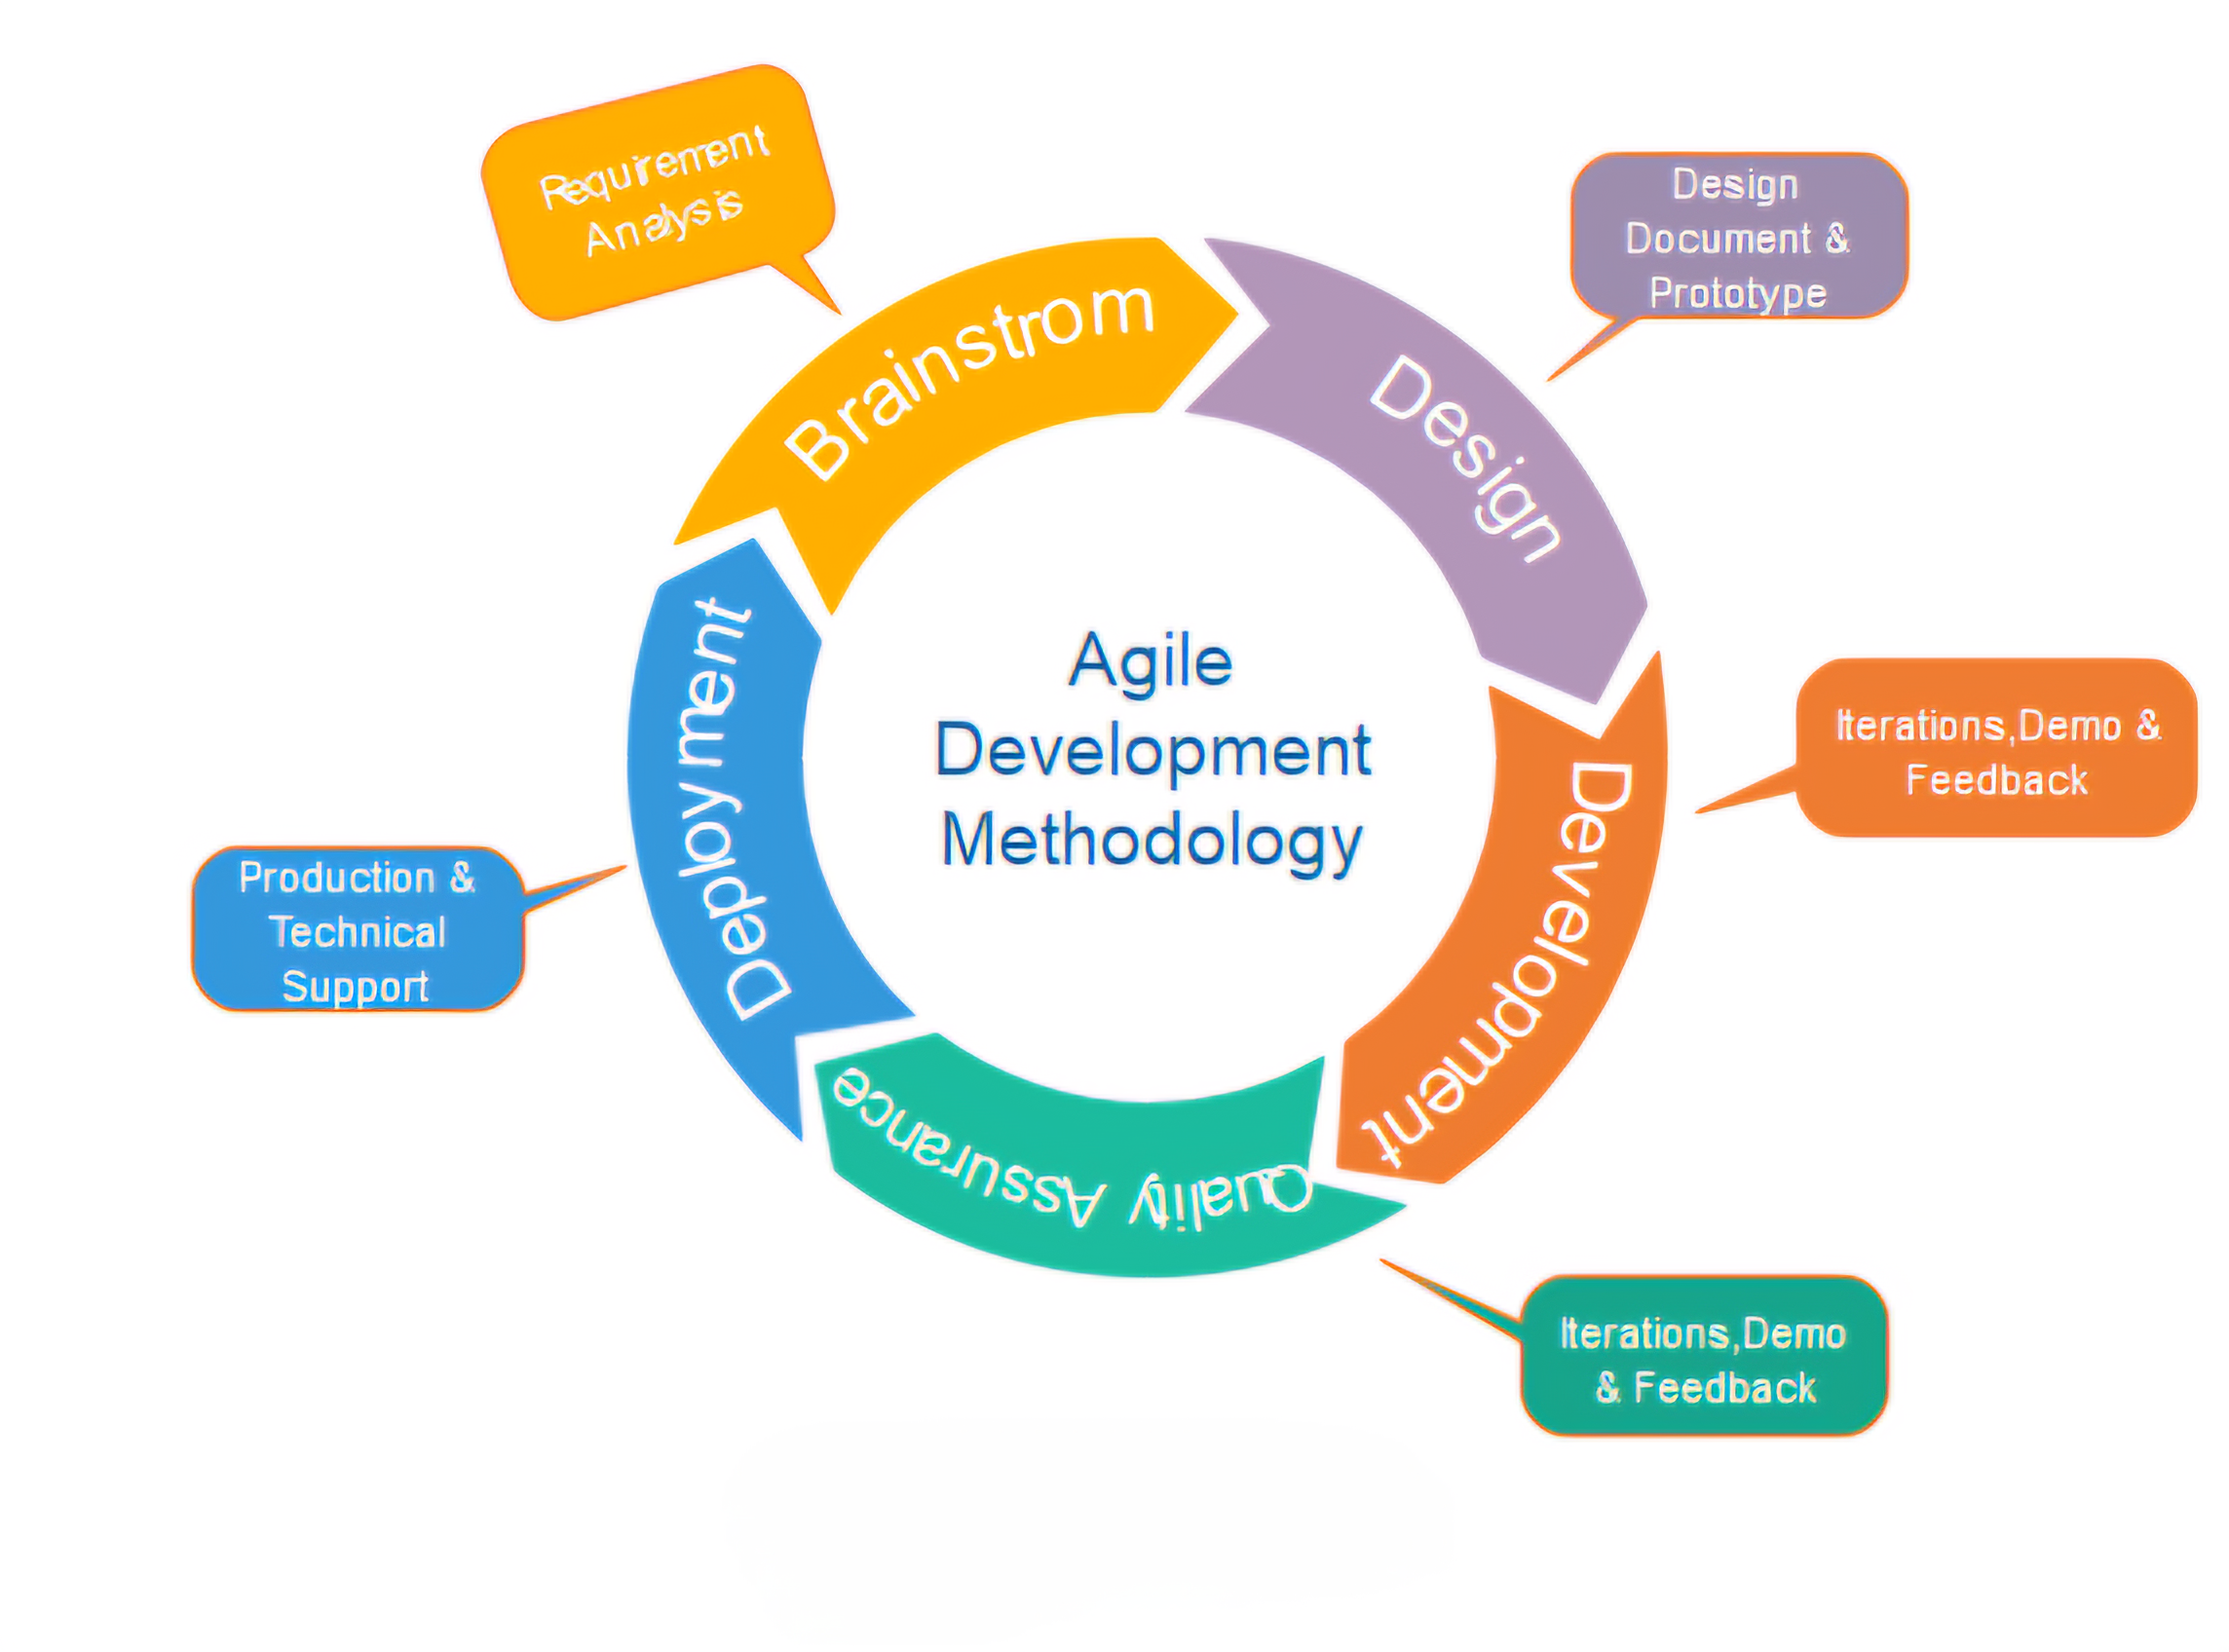
\includegraphics[scale=0.1]{img/agilemodel.png}
        \caption{Agile Development Model}
        \label{fig:agilemodel}
    \end{figure}
\subsection{Agile Sprints}

\subsubsection{Sprint 1: Project Definition and Dataset Exploration}
\textbf{Duration:} Initial Phase\\
\textbf{Goal:} Define the facial inpainting problem and identify suitable datasets for training and evaluation.

\textbf{Key Activities:}
\begin{itemize}
    \item Reviewed existing facial inpainting and image restoration methods.
    \item Explored publicly available face datasets suitable for training and evaluation.
    \item Identified the need to preserve facial structure, texture, and identity during reconstruction.
    \item Defined the main evaluation criteria, including image quality and identity preservation.
\end{itemize}

\textbf{Outcomes:}
\begin{itemize}
    \item Facial inpainting problem and project objectives were clearly defined.
    \item Suitable datasets and evaluation metrics were identified.
    \item Initial system requirements were established.
\end{itemize}


\subsubsection{Sprint 2: Dataset Preparation and Mask Generation}
\textbf{Duration:} Development Phase\\
\textbf{Goal:} Prepare the facial image dataset and generate masked training samples for different facial regions.

\textbf{Key Activities:}
\begin{itemize}
    \item Collected and prepared face images for model training and evaluation.
    \item Generated masks for important facial regions such as the eyes, nose, mouth, and eyebrows.
    \item Applied facial alignment and image resizing to obtain consistent input dimensions.
    \item Prepared masked and corresponding ground-truth image pairs for training.
\end{itemize}

\textbf{Outcomes:}
\begin{itemize}
    \item Training and evaluation data were prepared successfully.
    \item Region-specific facial masks were generated.
    \item The dataset was ready for LGNet training.
\end{itemize}


\subsubsection{Sprint 3: LGNet Architecture and Training Pipeline}
\textbf{Duration:} Development Phase\\
\textbf{Goal:} Design and implement the LGNet-based facial inpainting pipeline.

\textbf{Key Activities:}
\begin{itemize}
    \item Designed the local and global context modules for facial feature reconstruction.
    \item Integrated facial masks and landmark information into the model input.
    \item Implemented the multi-objective loss combining L1, perceptual, style, identity, and landmark losses.
    \item Configured the PyTorch training pipeline with mixed-precision training.
\end{itemize}

\textbf{Outcomes:}
\begin{itemize}
    \item LGNet training architecture was implemented.
    \item The complete training pipeline was successfully configured.
    \item Initial training runs confirmed that the model could reconstruct masked facial regions.
\end{itemize}


\subsubsection{Sprint 4: Model Training and Optimization}
\textbf{Duration:} Training Phase\\
\textbf{Goal:} Train LGNet and improve reconstruction quality while maintaining facial identity.

\textbf{Key Activities:}
\begin{itemize}
    \item Trained the model using PyTorch automatic mixed precision across multiple epochs.
    \item Monitored training and validation losses to evaluate convergence.
    \item Adjusted the training configuration based on observed model performance.
    \item Saved model checkpoints and selected the best-performing checkpoint for evaluation.
\end{itemize}

\textbf{Outcomes:}
\begin{itemize}
    \item Training loss decreased consistently throughout training.
    \item The model reached stable convergence without significant overfitting.
    \item The fifth-epoch checkpoint was selected as the final model checkpoint.
\end{itemize}


\subsubsection{Sprint 5: Boundary Blending and Identity Preservation}
\textbf{Duration:} Refinement Phase\\
\textbf{Goal:} Improve the visual quality of reconstructed regions and preserve the identity of the input face.

\textbf{Key Activities:}
\begin{itemize}
    \item Implemented alpha feathering to reduce visible boundaries around reconstructed regions.
    \item Applied Poisson blending to improve colour and illumination consistency.
    \item Used facial identity embeddings to evaluate identity preservation.
    \item Verified facial landmark consistency between reconstructed and original images.
\end{itemize}

\textbf{Outcomes:}
\begin{itemize}
    \item Boundary artifacts were reduced after post-processing.
    \item Reconstructed regions achieved better visual and structural consistency.
    \item Identity preservation was incorporated into the final evaluation process.
\end{itemize}


\subsubsection{Sprint 6: Evaluation and Comparative Analysis}
\textbf{Duration:} Final Phase\\
\textbf{Goal:} Evaluate the final model and compare its performance with the LaMa baseline.

\textbf{Key Activities:}
\begin{itemize}
    \item Evaluated the final model on the held-out test samples.
    \item Computed PSNR, SSIM, LPIPS, RMSE$_{\log}$, FID, and ArcFace identity scores.
    \item Analysed performance separately for different facial regions.
    \item Compared LGNet results with the LaMa baseline using the stored evaluation metrics.
\end{itemize}

\textbf{Outcomes:}
\begin{itemize}
    \item Final quantitative results were obtained for the proposed model.
    \item LGNet showed strong reconstruction quality and identity preservation.
    \item The final system and evaluation results were prepared for demonstration and reporting.
\end{itemize}

% \newpage
\section{Model Deployment}

This section describes the deployment of the MorphAI system, including the
frontend interface, backend services, trained LGNet model, and the complete
inference pipeline.

\subsection{Frontend Development}

The frontend was developed using React to provide a simple interface for
uploading a facial image and selecting the region to be reconstructed. The
main components include:

\begin{itemize}
    \item Facial image upload with image preview.
    \item Selection of facial regions such as the eyes, nose, eyebrows, and mouth.
    \item Display of the reconstructed facial image.
    \item Before-and-after comparison of the input and generated images.
    \item Status messages for image processing and inference.
\end{itemize}

\noindent Screenshots of the user interface are provided in
Appendices~\ref{app:C1}.

\subsection{Backend Development}

The backend was implemented using Flask to handle image processing and model
inference. Its main responsibilities include:

\begin{itemize}
    \item Receiving the uploaded facial image and selected facial region.
    \item Extracting facial landmarks using the landmark extraction module.
    \item Generating a region-specific mask for the selected facial area.
    \item Creating the facial landmark heatmap required by the model.
    \item Combining the RGB image, mask, and heatmap to form the five-channel
    model input.
    \item Running inference using the trained LGNet generator.
    \item Applying boundary blending to reduce visible seams around the
    reconstructed region.
    \item Returning the final reconstructed image to the frontend.
\end{itemize}

\subsection{Model Integration}

The trained LGNet generator was integrated into the backend for real-time
facial inpainting. The complete inference process follows these steps:

\begin{itemize}
    \item The user uploads an image and selects a facial region.
    \item The backend extracts facial landmarks and generates the corresponding mask.
    \item The RGB image, mask, and landmark heatmap are combined into the
    required five-channel input.
    \item LGNet generates the reconstructed facial region.
    \item Boundary blending is applied to obtain a visually seamless result.
    \item The reconstructed image is returned to the React frontend for display.
\end{itemize}

\noindent The system can additionally use the identity extraction module to
compare the reconstructed face with the original face using facial embeddings.
This helps verify whether the reconstructed result preserves the identity of
the input subject.

\noindent Overall, the deployment integrates the React frontend, Flask backend,
facial preprocessing modules, and LGNet generator into a single end-to-end
facial inpainting system.